\section{Zielsetzung}
Es sollen die Halbwertzeiten von verschiedenen radioaktiven Isotopen bestimmt werden.
\section{Theorie}
Stabile Atomkern sind sie nur, wenn das Verhältnis zwischen Neutronen- und Protonanzahl innerhalb eines engen Grenzens
liegen.
Je nach Nuklid ist die Neutronenanzahl bis zu 50 \% höher im Kern vorhanden als Protonen.
Aus diesem Zahlenverhältnis, außerhalb der Stabilitätsgrenze, zerfallen sie mit unterschiedlicher Wahrscheinlichkeit
solange bis das Nuklid wieder stabil ist.
Die Zerfallswahrscheinlichkeit wird auch als Halbwertzeit $T_(\frac{1}{2})$ genannt und beschreibt
die Zeitspanne in welcher Größe und Aktivität das Startnuklid um die Hälfte gesunken ist.
Die Halbwertzeit $T_(\frac{1}{2})$ variiert sich von Sekunden bis zu Jahren je nach Nuklid.
Zur Herstellung von radioaktiven Isotopen werden stabile Atomkerne mit Neutronen beschossen.
Dringt ein Neutron in einen Atomkern ein, so wird es Zwischenkern oder Compoundkern genannt.
Beim Eindringen verteilt sich die Energie auf die große Anzahl der Nukleonen im Kern und ist nun instabil.
Da die kinetische Energie des Neutrons ein Nukleon abzustoßen zu gering ist, geht der angeregte Zwischenkern durch
Emission eines $\gamma$-Quant wieder in den Grundzustand zurück.
Der neu entstandene Kern ist langlebiger als der Zwischenkern und wandelt sich unter $\beta$-Strahlung in einen stabilen
Kern um.
\begin{equation*}
  \ce{^{m+1}_{Z}A  -> ^{m-1}_{Z-1}C + e +E _{\text{kin}}+ \bar{\symup{\nu}}_e}
\end{equation*}
Dabei ist $\overline{v_e}$ ein Antineutrino.
Das sogenannte Wirkunsquerschnitt $\sigma$ beschreibt die Wahrscheinlichkeit für die Reaktion eines Neutrons mit einem stabilen Kern.
Es beschreibt eine Fläche, die so groß ist, dass das treffende Neutron vom Kern eingefangen werden müssen.
Dabei ist sie stark von der Geschwindigkeit $v$ und somit auch von ihrer kinetischen Energie des Neutrons abhängig.
Da das Neutron als freies Teilchen in der Natur nicht vorkommt wird sie durch eine Kernreaktion erzeugt.
Dafür werden Beryllium Kerne mit Alphastrahlen, die aus dem radioaktiven Zerfall von $\ce{^{226}_{}Ra}$ kommen, beschossen. Es folgt nun folgende Reaktion ab:
\begin{equation*}
    \ce{^{9}_{4}Be + ^{4}_{2}$\alpha$ -> ^{12}_{6}C + ^1_0n}
\end{equation*}
Die dabei entstandenen Neutronen haben ein kontinuierliches Energiespektrum bis zu 13,7 MeV. Um die Energie der Neutronen zu verringern, werden sie durch eine
dicke Materieschicht geschickt. Es treten dabei elastische Stöße auf, dabei soll die
Materien-Kerne so gewählt sein, dass sie von der Masse gleich der Neutronen ähneln.
Nun werden Proben mit Neutronen bestrahlt und durch einen $\beta$-Zerfall in stabile Isotope gebracht.
Der radioaktive Zerfall verläuft exponentiell und beschreibt die noch nicht zerfallenen Kerne zu einem Zeitpunkt $t$ durch die Formel:
\begin{equation}
  N(t)= N_0 e^{-\lambda t}
  \label{eq:1}
\end{equation}
$N_0$ bedeutet die zur Zeit $t = 0$ vorhanden instabile Kerne und $\lambda$ die Zerfallskonstante, welches die Aussage über die Wahrscheinlichkeit
des vorliegenden Zerfalls macht.
Die Halbwertzeit $T_{\frac{1}{2}}$ ergibt nun mit der Formel:
\begin{equation}
  T_{\frac{1}{2}} = \frac{\ln 2}{\lambda}
  \label{eq:2}
\end{equation}
Ein anderer und einfacher Weg zur Bestimmung der noch vorhandenen Kerne ist
ein genau definierter Zeitintervall $\delta t$.
Da $\delta t$ ebenfalls zeitabhängig ist lässt sich die Beziehung aus der Formel (\ref{eq:1})
nun diese Formel herleiten:
\begin{equation}
  N_{\delta t} (t) = N(t) - N(t+\delta t) \Rightarrow N_{\delta t} (t) =N_0 (1-e^{-\lambda \delta t}) \cdot e^{-\lambda t}
  \label{eq:3}
\end{equation}
Problematisch bei diesem Weg ist die Wahl eines geeigneten Zeitintervalls $\delta t$. Ist sie zu klein folgt ein großer statistischer Fehler.
Ist sie zu große so bekommt $\lambda$ einen systematischen Fehler.
\begin{figure}
  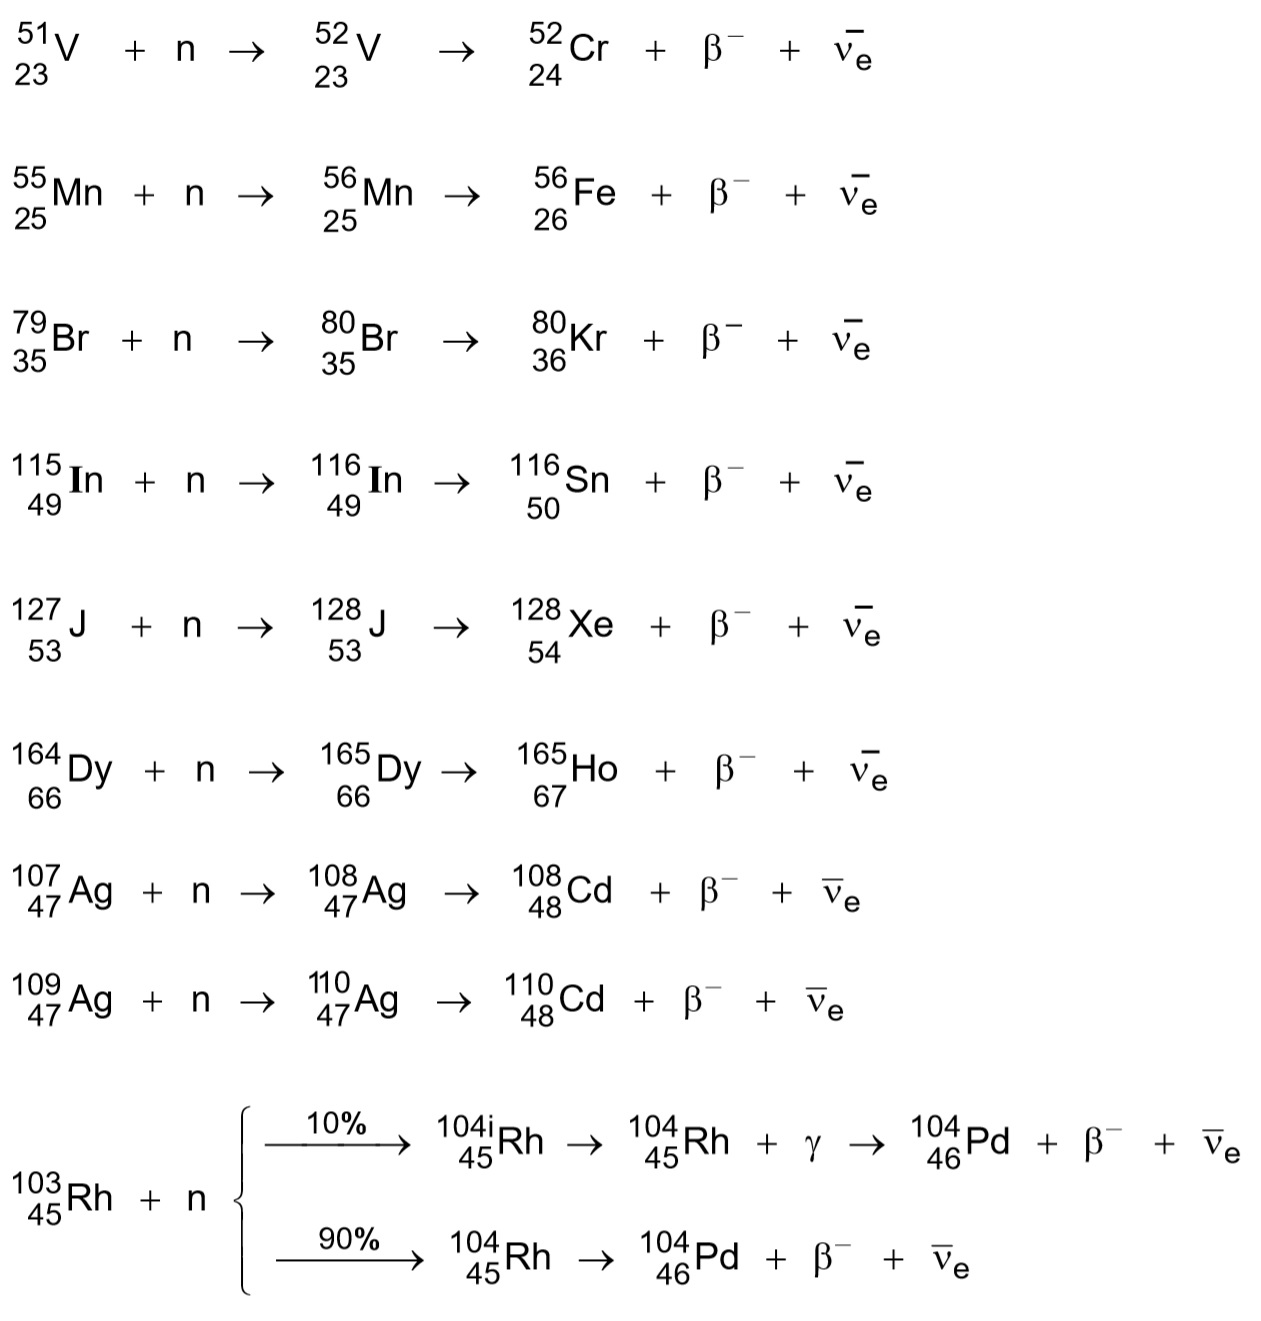
\includegraphics[width=\textwidth]{content/Verlauf.jpg}
  \caption{Verschiedene Zerfallsreihen \cite{1}.}
  \label{abb:1}
\end{figure}
In Abbildung (\ref{abb:1}) fällt auf, dass die Zerfallsreihe $\ce{^{103}_{45}Rh}$ mit unterschiedlicher Wahrscheinlichkeit
in zwei verschiedenen instabile Isotope fällt.
Diese beiden Zerfälle laufen mit unterschiedlichen Halbwertzeiten $T_{\frac{1}{2}}$ gleichzeitig statt.
